% !TEX root = MAIN.tex

\STARTCHANGEDWPT
\section{INTEGRATION WITH ECSS PRACTICES}
\label{sec:isvv}
To discuss applicability of mutation testing (i.e., code-driven or data-driven) to different test levels (i.e., unit, integration, system, acceptance), we provide a generic overview of the interactions typically stressed by different test levels. Unit test cases focus on interactions within single units (e.g., functions belonging to a same source files) or few units belonging to a same component. Integration test cases trigger interactions between distinct units or multiple components. System test cases exercise interactions between all the components of the system.
Figure~\ref{fig:mutationTestingVSTestingLevels} provides a generic overview of the interactions typically stressed by different test levels

According to ECSS standards, system test cases might be executed on a host system with emulated hardware. Acceptance test cases exercise all the system components but in the operational environment. For this reason, mutation testing cannot be adopted in the context of acceptance testing because the deployment of multiple version of the system (one for each mutant) might be particularly expensive and may lead to safety hazards.

\begin{figure}[h]
  \centering
    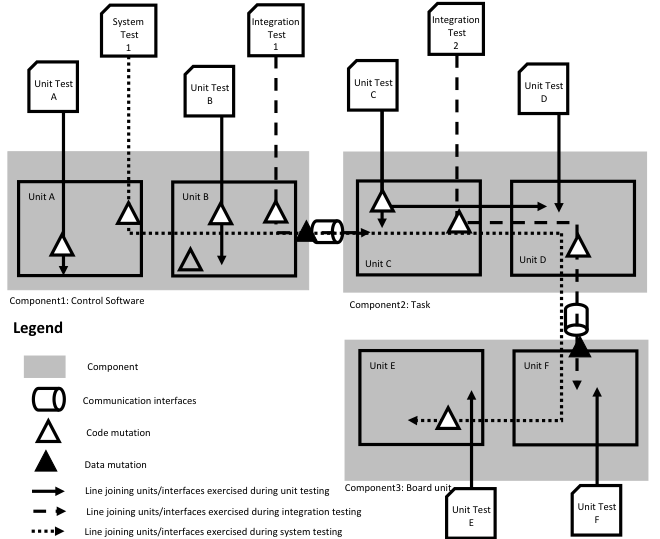
\includegraphics[width=10cm]{images/TestingLevels}
      \caption{Mutation Testing Approaches for Different Testing Levels.}
      \label{fig:mutationTestingVSTestingLevels}
\end{figure}

%Test suite evaluation through code-driven mutation testing appear to be feasible for all the testing levels (i.e., unit, integration, and system), except acceptance testing for the reasons mentioned above.

\INDEX{Unit testing} is the typical scenario in which code-driven mutation testing is adopted in other contexts, for this reason it should be targeted also in the case of space software.
In addition, code-driven test generation approaches based on static program analysis can be adopted to automatically generate unit test cases.
Data-driven mutation techniques, instead, are unlikely to be useful in the context of unit testing.
Indeed, Unit test cases do not verify the interaction between units but rely on stubs when the testing of a unit requires the interaction with another component.
% Also, although certain units focus on the communication with hardware components (e.g., chips) applying data-driven mutation techniques in that context would simply lead to a form of robustness testing targeting hardware components.

In the context of \INDEX{integration testing}, the use of traditional code-driven mutation operators conceived for unit testing may lead to an inadequate assessment of the test suite quality.
Indeed, an integration test suite is not expected to detect functional problems of single units; for this reason, the mutation score for an integration test suite computed with mutation operators for functional faults (e.g., the sufficient set) may not adequately measure the quality of the test suite.
% The adoption of operators dedicated to integration testing might be evaluated instead~\cite{grechanik2016mutation,delamaro2001proteum}; however, these approaches target API methods but they do not inject higher level errors (e.g., errors in the structure of the data generated by multiple components).
For this reason, in FAQAS, we suggest to rely on data-driven mutation testing to assess the quality of integration test suites.

% Test case generation approaches based on static analysis may be used, in principle, to support the generation of test cases that kill data-driven mutants; however, to date, the manual implementation of missing test cases remains the most appropriate solution  (see Section~\ref{sec:data:test_suite_augmentation}).


In the context of \INDEX{system testing}, both code-driven and data-driven mutation can be applied. However, the long execution time required by system test cases may emphasize the scalability problems of mutation testing; the evaluation of solutions for such scalability problems are part of the FAQAS objectives.
%However, within FAQAS, we expect to develop solutions that will enable mutation testing to scale with large system test suites.
Depending on the development process, system-level test cases may focus only on specific features of the system under test; for this reason, system-level test cases may not reach 100\% statement coverage. For the same reason, system-level test cases may lead to a mutation score that is lower than the one achieved with unit test cases.

We suggest to compute the mutation score by considering all the available test suites (i.e., a mutant is killed if at least one test case of any available test suite fails).
% Although software testing literature report results that show the feasibility of relying on model-based test generation to automatically generate system level test suites (see Deliverable D1), such approaches are preliminary and will not be evaluated in the context of FAQAS. In the context of FAQAS, we do not aim to automatically generate system-level test cases.

\begin{figure}[h]
  \centering
    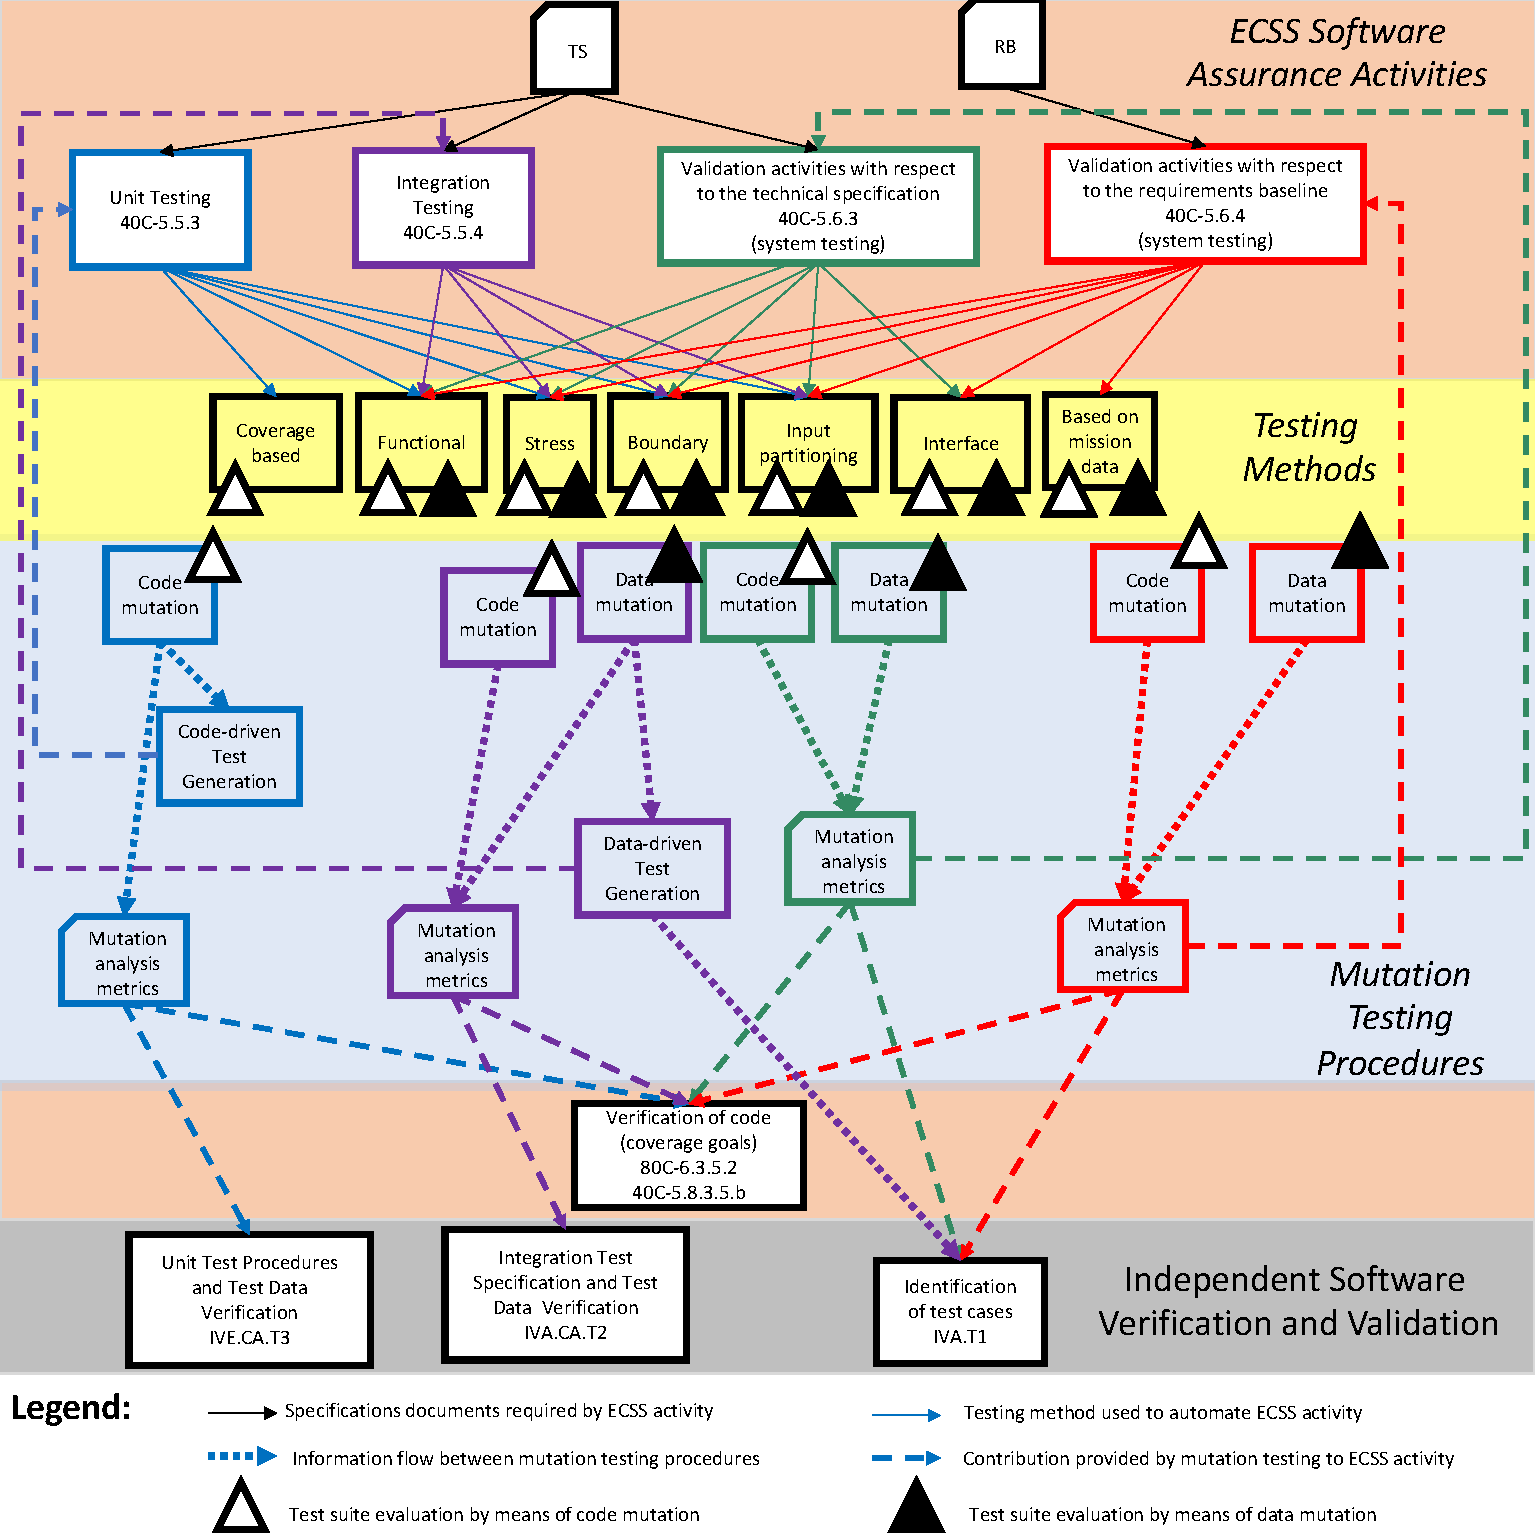
\includegraphics[width=0.9\textwidth]{images/ECSSTesting}
      \caption{Relations between ECSS activities and activities of the mutation testing process.}
      \label{fig:ECSSTesting}
\end{figure}

Figure~\ref{fig:ECSSTesting} shows the envisioned relationships between ECSS software testing practices and the main activities of the mutation testing process (i.e., code mutation, data mutation, code-based generation, model-based generation, and generation of the mutation score). These relationships guide the definition of a mutation testing process integrated with ECSS standards.

% In Figure~\ref{fig:ECSSTesting}, black arrows show the specifications documents (i.e., Technical Specifications and Requirement Baselines) used to support ECSS testing activities (i.e., Unit Testing, Integration Testing, Validation activities with respect to the technical specification and Validation activities with respect to the requirements baselines). Colored arrows are used to associate ECSS activities to specific testing methods suggested in the ECSS standard (e.g., mission data is used for ECSS-E-ST-40C-5.6.4). Triangles are used to indicate which type of mutation testing (i.e., code-driven or data-driven) is likely applicable when a specific testing method is applied. White triangles are used to indicate that code mutation can be applied with a certain testing method, black triangles are used for data mutation.

% Concerning the type of mutation activity associated to each testing method, we observe that although code-driven mutation might be used for all the testing methods in use, it is unlikely to be adopted when mission data is used for testing, because mission data might lead to long software executions that cannot be repeated for all the mutants. Data-driven mutation, instead, is unlikely to be used with coverage based testing which often targets unit tests.

Test case generation based on static analysis can be used in the context of unit and integration testing for both code-driven and data-driven mutation testing. In the system testing context, model-based generation might be adopted; however, it is not covered by FAQAS.

% In Figure~\ref{fig:ECSSTesting}, dashed arrows show how the mutation testing procedures can contribute to ECSS activities. The mutation score computed by the mutation testing process might be used to support verification activities; more precisely, it might be used as an additional coverage metric for the activities described in ECSS-Q-ST-80C 6.3.5.2 and ECSS-E-ST-40C 5.8.3.5.b. Independent Software Verification and Validation~\cite{ESAISVV} can benefit from the mutation testing process as well. The mutation score can support Unit Test Procedures and Test Data Verification (IVE.CA.T3 in~\cite{ESAISVV}) and Integration Test Specification and Test Data Verification (IVA.CA.T2 in~\cite{ESAISVV}). Finally, model-based test generation and mutation score will support ISVV during the identification of test cases (IVA.T1 in~\cite{ESAISVV}).

\ENDCHANGEDWPT
